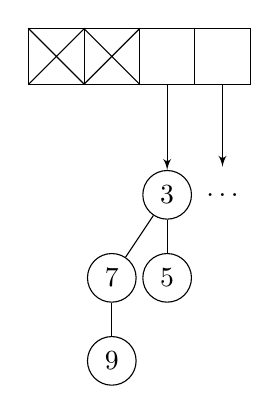
\begin{tikzpicture}
\usetikzlibrary{shapes.misc, arrows}

\node [draw = black, minimum size = 2em] (list0) at (0em, 0em) {};
\node [draw = black, minimum size = 2em, cross out] at (0em, 0em) {};
\node [draw = black, minimum size = 2em] (list1) at (2em, 0em) {};
\node [draw = black, minimum size = 2em, cross out] at (2em, 0em) {};
\node [draw = black, minimum size = 2em] (list2) at (4em, 0em) {};
\node [draw = black, minimum size = 2em] (list3) at (6em, 0em) {};



\node [shape = circle, minimum size = 1.5em] (t3) at (6em, -5em) {$\ldots$};
\path [draw, -latex'] (list3.south) -- (t3);

\node [draw = black, shape = circle, minimum size = 1.5em] (ins0) at (4em, -5em) {$3$};
\node [draw = black, shape = circle, minimum size = 1.5em] (ins1) at (4em, -8em) {$5$};
\path [draw] (ins0) -- (ins1);

\node [draw = black, shape = circle, minimum size = 1.5em] (ins2) at (2em, -8em) {$7$};
\node [draw = black, shape = circle, minimum size = 1.5em] (ins3) at (2em, -11em) {$9$};
\path [draw] (ins0) -- (ins2);
\path [draw] (ins2) -- (ins3);

\path [draw, -latex'] (list2.south) -- (ins0);

\end{tikzpicture}